%% Template for ENG 401 reports
%% by Robin Turner
%% Adapted from the IEEE peer review template

\documentclass[peerreview]{IEEEtran}
\usepackage{cite} % Tidies up citation numbers.
\usepackage{url} % Provides better formatting of URLs.
\usepackage[utf8]{inputenc} % Allows Turkish characters.
\usepackage{booktabs} % Allows the use of \toprule, \midrule and \bottomrule in tables for horizontal lines
\usepackage{graphicx}
\usepackage{xcolor}
\usepackage{microtype}

\graphicspath{{./graphics}}

\begin{document}
\title{System on Chip Architecture \\ WSS Project Report}

\author{Brignone Giovanni \\ Castagneri Dario \\ Paganini Giovanni}
\date{\today}

\maketitle
\tableofcontents
\listoffigures

\IEEEpeerreviewmaketitle
\begin{abstract}
	\emph{Well-being Station} is a system able to control indoor environment
	parameters to keep them within \emph{Comfort Zones}~\cite{leudsen_freymark}
	while at the same time minimizing the consumed energy.
	The logic was implemented in software and it is an infinite iteration of:
	sensing (temperature and humidity, both indoor and outdoor), controlling
	(elaborate sensed data and control environment conditioning devices
	accordingly) and wait.
	The underlying hardware is mainly composed of an \emph{STMicroelectronics
	STM32F4} board, a couple of temperature and humidity sensors and a set
	of relays used to control environment conditioning devices.
	In \emph{High Quality Mode} the system uses all the devices it has at its
	disposal to reach the \emph{Comfortable Zone}, while in \emph{ECO Mode}
	the system trades-off between comfort and energy consumption.

\end{abstract}

\section{Introduction}
Nowadays indoor environment conditioning is mostly based on indoor temperature
only: this is not optimal both in terms of comfort (which depends on other
parameters too, such as air humidity) and in terms of power consumption.
The \emph{Well-being Station} is therefore aimed at addressing both of these issues,
exploiting Leudsen and Freymark studies about human comfort~\cite{leudsen_freymark}
and smart controlling of an heterogeneous set of environment conditioning devices,
basing decisions on both indoor and outdoor environment conditions.

\section{Background}
Indoor climate is influenced by a large number of parameters. The most
important are air humidity and temperature, temperature of the walls and the
floor, air velocity. Thermal comfort is reached whenever there is:
\begin{enumerate}
	\item balance between the heat produced by the body and the
		amount of heat lost from the body.
	\item thermal neutrality between the skin and the body core temperatures~\cite{indoor_comfort}. 
\end{enumerate}
In order to get such balances, the main exploitable factors are air temperature
and relative humidity.

\subsection{Leudsen-Freymark Comfort Zones}
Even if the thermal comfort is highly subjective, it is possible to estimate
comfort conditions according to physical air parameters.
Leudsen and Freymark studies about indoor human comfort led to the definition of
different \emph{Comfort Zones} on the \emph{Air Temperature} $\times$
\emph{Relative Humidity} plane, as shown in Figure~\ref{fig:lf_plot}.
In particular there are three zones:
\begin{itemize}
	\item \emph{Comfortable}: ideal conditions
	\item \emph{Still Comfortable}: fine conditions, at the boundary between
		ideal and to avoid conditions
	\item \emph{Uncomfortable}: conditions which should be avoided
\end{itemize}

\begin{figure}[!htbp]
	\centering
	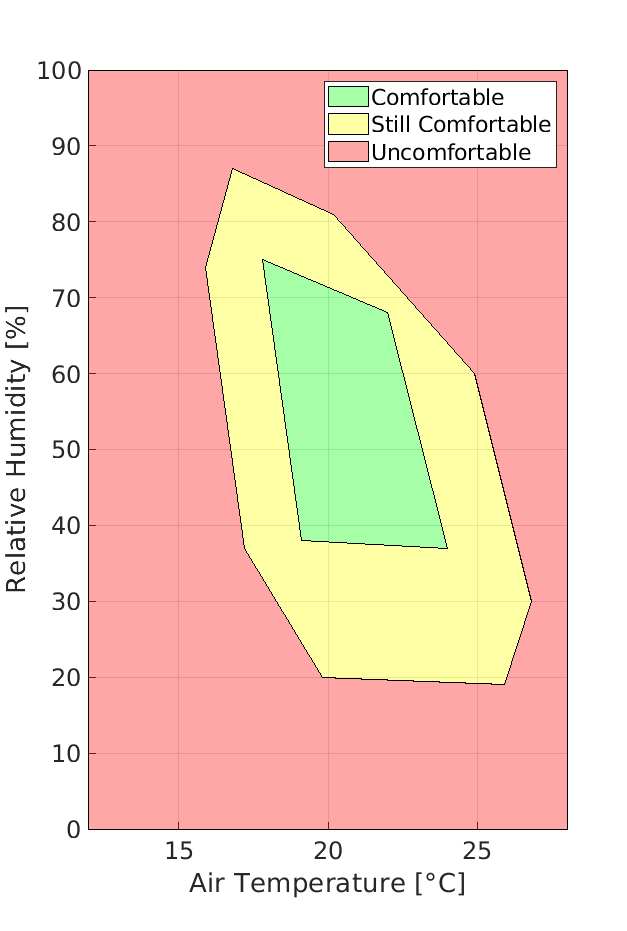
\includegraphics[width=0.7\columnwidth]{leudsen_freymark_plot} 
	\caption{Leudsen-Freymark \emph{Comfort Zones} plot}
	\label{fig:lf_plot}
\end{figure}

It is evident that extreme conditions for both temperature and humidity can
cause uncomfortable feelings.

\subsection{Point Inclusion in Polygon Test}
The problem of determining the \emph{Comfort Zone} at which the environment is,
knowing the actual \emph{Air Temperature} $T$ and \emph{Relative Humidity} $H$,
can be reduced to the test of inclusion of point $(T,H)$ first within the
\emph{Comfortable} and then \emph{Still Comfortable} polygons.

A linear-complexity solution of this problem is provided by the
\emph{PNPOLY}~\cite{pnpoly_2021} algorithm.

\subsection{Environment Conditioning Devices}
In order to move environment conditions throughout the Leudsen-Freymark plane
it is possible to exploit different devices:
\begin{itemize}
	\item \textbf{Active}:
		\begin{itemize}
			\item \emph{Temperature} conditioning: they can be both
				heaters and coolers; they are typically the
				most power-hungry devices.
			\item \emph{Humidity} conditioning: they can be both
				humidifiers and dehumidifiers.
		\end{itemize}
	\item \textbf{Passive}:
		\begin{itemize}
			\item \emph{Temperature} and \emph{Humidity} conditioning:
				they are automated windows; they consume almost
				no power (the energy for opening and closing can
				be neglected), but their effectiveness highly
				depends on outdoor conditions.
		\end{itemize}
\end{itemize}

\section{Proposed Solutions}
The proposed design of the \emph{Well-being Station} is a mix of hardware and software.
\subsection{Hardware}
Figure~\ref{fig:hw} shows the schematics of the hardware architecture.
\begin{figure}[!htbp]
	\centering
	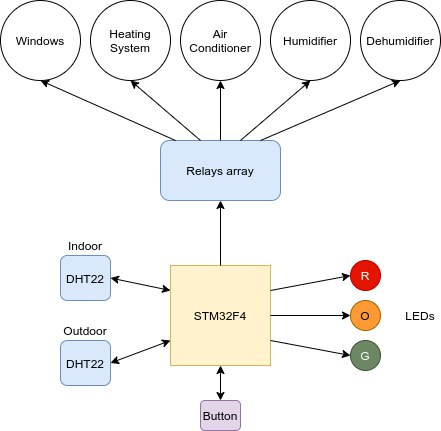
\includegraphics[width=0.7\columnwidth]{hw} 
	\caption{Hardware architecture schematics}
	\label{fig:hw}
\end{figure}
\subsubsection{Computing}
it is composed of a microcontroller used for running the software and interfacing
with the other hardware components. In our specific implementation an
\emph{STMicroelectronics STM32F407} board have been used.
\subsubsection{Sensing}
it is composed of sensors used to sample temperature and humidity (one indoor
and one outdoor). In our specific implementation 2 \emph{DHT22} sensors have been
used.
\subsubsection{Actuating}
it is composed of one relay for each \emph{environment conditioning device}.
\subsubsection{I/O}
it is composed of a \emph{button}, allowing the user to switch the
\emph{Operating Mode}, and a set of \emph{LEDs}, used to inform the user about
the current \emph{Comfort Zone} (green $\rightarrow$ \emph{Comfortable}, orange
$\rightarrow$ \emph{Still Comfortable}, red $\rightarrow$ \emph{Uncomfortable}).
\subsection{Software}
The software stack is made up of different components which are described in
following Subsections.

The main function is including an infinite loop calling the \emph{Controller}
at regular intervals.

\bigskip
\subsubsection{Controller}
it is the most relevant part of the design: it is in charge of taking decisions
according to \emph{operating mode} and \emph{environment conditions}.

The currently supported \emph{Operating Modes} are:
\begin{itemize}
	\item \textbf{High Quality} (\emph{HQ}): if the current \emph{Comfort Zone}
		is different from \emph{Comfortable} all useful \emph{active
		conditioning devices} are activated, as shown in
		Figure~\ref{fig:hq_act}.
	\item \textbf{Power Saving} (\emph{ECO}): if the current \emph{Comfort
		Zone} is different from \emph{Comfortable} it activates
		\emph{passive conditioning devices} if possible (e.g.\ if indoor
		temperature is too hot and outdoor temperature is lower than
		indoor windows are opened).
		If it is not possible to exploit \emph{passive devices} and the
		environment is \emph{Uncomfortable} \emph{active devices} are
		activated, prioritizing less power-hungry devices, as shown in
		Figure~\ref{fig:eco_act} (heaters/coolers are activated only when
		strictly necessary to reach \emph{Still Comfortable} zone, since
		they are more power-hungry).
	\item \textbf{Not Active} (\emph{OFF}): all conditioning devices are
		turned off.
\end{itemize}
\begin{figure}[!htbp]
	\centering
	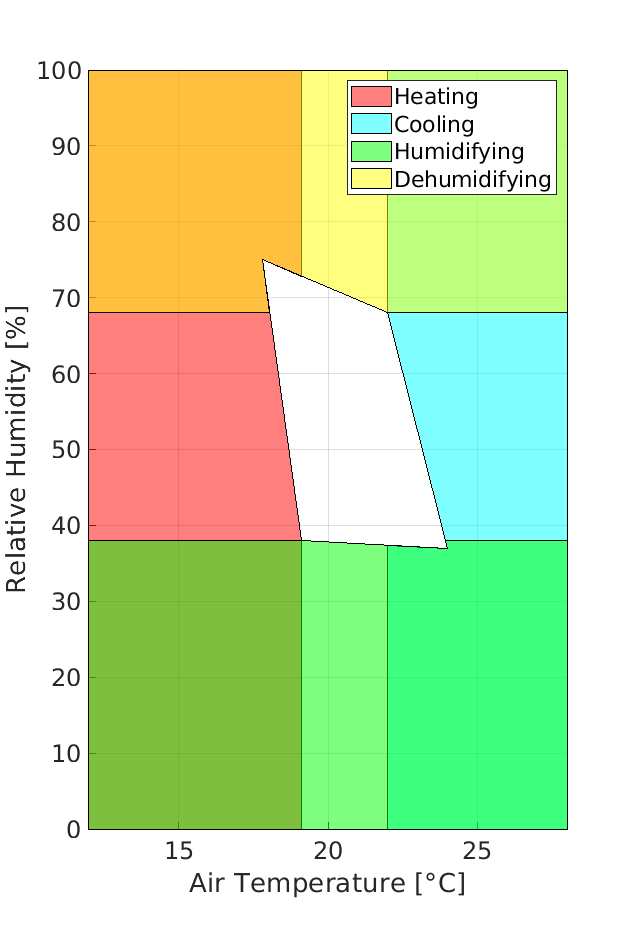
\includegraphics[width=0.7\columnwidth]{comfort_actions} 
	\caption{Devices enabling in \emph{HQ} mode}
	\label{fig:hq_act}
\end{figure}
\begin{figure}[!htbp]
	\centering
	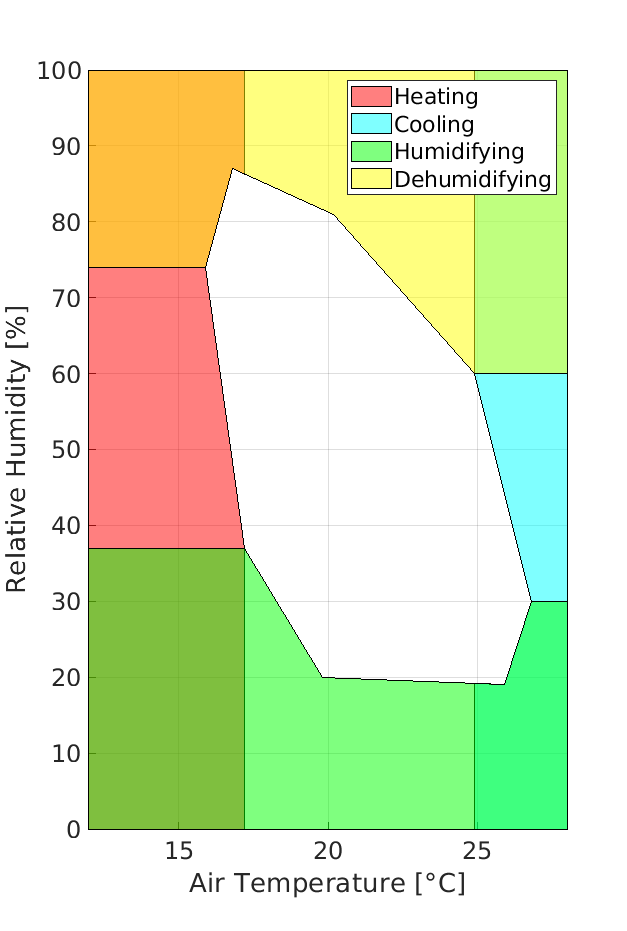
\includegraphics[width=0.7\columnwidth]{still_comfort_actions} 
	\caption{Active devices enabling in \emph{ECO} mode}
	\label{fig:eco_act}
\end{figure}
\subsubsection{Comfort}
it is in charge of determining the \emph{Comfort Zone} of a generic
$(temperature, humidity)$ point, exploiting the \emph{PNPOLY} algorithm.
\subsubsection{Drivers}
in order to drive different external peripherals, there are several source files, that 
receive commands from \emph{Controller} and relies on low level \emph{STM HAL library}.
In particular we have:
\begin{itemize}
	\item \textbf{Button}: it implements
		\texttt{GPIO\_EXTI\_Callback} (catch the button press, starting
		the timer and disabling further interrupts) and \emph{TIMER2}
		\texttt{PeriodElapsedCallback} (debounce, checking for the
		effective GPIO pin status and re-enabling interrupts at the end).
	\item \textbf{DHT}: it is used to perform sensor data reading and support
		both \emph{DHT11} and \emph{DHT22}. In particular, due to the
		non-standard and custom communication protocol, it performs a
		sort of initialization, switching the output up and down for a
		given time, and then waits for the value in input. The detailed protocol
		is shown in Figure~\ref{fig:dht_timing}
	\item \textbf{DWT}: this library relies on the \emph{SysTick Debug Timer}
		and it is used to exploit microseconds delays, not natively
		supported by the \emph{HAL Library}.
	\item \textbf{Debug}: it is used to print debug strings on the UART console 
        and it relies on the \texttt{HAL\_UART\_Transmit} function.
	\item \textbf{RTC}: this library implements both the RTC event callbacks,
	    \texttt{HAL\_RTC\_AlarmA} and \texttt{HAL\_RTCEx\_AlarmB},
	    in order to switch mode automatically between day and night.
	\item \textbf{Relay}: it offers functions to initialize and control relays.
	\item \textbf{StatusLED}: it implements functions to control an array of
		LEDs, simply passing the desired level (\texttt{Off}, \texttt{Low},
		\texttt{Medium}	and \texttt{High}).
\end{itemize}

\section{Possible applications}
\emph{Well-being Station} has very wide application fields. It can be integrated
in a positive cooperation with any heating and cooling systems of any private or
public buildings. Whenever required, it maintains a proper level of indoor
comfort in terms of ideal temperature and humidity in an efficient and
eco-friendly way.

\section{Results and discussion}
In order to perform firmware and, more in general, a complete system analysis,
we have decided to divide the development and test phases in two different parts.
\subsection{Renode Simulation}
	During this phase, we have used the simulation environment provided by 
	\emph{Renode}~\cite{renode}. In particular, we have maily focused on adding 
	new functionalities and we have checked for the correctness of the controller
	logic. In order to reproduce the DHT sensors behaviour, we have injected
	temperature and humidity, both indoor and outdoor, directly into memory
	during debug. Renode has been exploited to simulate the user button, too,
	thanks to the \emph{PressAndRelease} function, that let us switching
	between different operating modes. Finally, we've use the UART console 
	offered by the \emph{showAnalyzer sysbus.uart1} command to print out some 
	demonstrative or diagnostic strings and to emulate the action of external
	LED and relays arrays.
	
	\subsection{Real Board Implementation}
	In this second phase, we have ported all the system to the real hardware, a
	\emph{DevEBox}~\cite{devebox} board based on the same microcontroller chosen
	as target. The overall system behaved as expected, but we had troubles with
	some external peripherals. In particular, the interaction with real DTH sensors
	was	tricky due to their particular custom communication protocol, based on
	strict timing for control signals, as shown in Figure~\ref{fig:dht_timing}.

	\begin{figure}[!htbp]
		\centering
		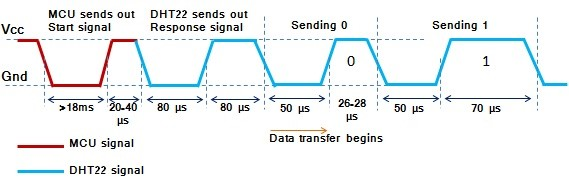
\includegraphics[width=0.9\columnwidth]{dht_timing} 
		\caption{DHT Data Read Protocol Timing}
		\label{fig:dht_timing}
	\end{figure}

	We also had to deal with a very important bounce effect, probably caused by
	the poor quality of the micro switch itself. Other peripherals, such as the
	LEDs and relays	arrays, worked smoothly, with only few adjustments needed
	with the respect to the board pinout. In any case, in this step we have
	mainly focused on the dependability of the different modules and on the
	stability of whole system, checking for the correctness of read data and
	corresponding behaviour of the outputs in a real environment. 

\section{Conclusions and Future Works}
\emph{Well-being Station} tries to provide a possible solution to the control of
indoor parameters, in particular temperature and humidity, in order to supply
the most comfortable conditions with special attention to the power consumption
and by consequence to the environment. As said, the firmware has been first tested
by simulation and then largely tried on a real board, as shown in as shown in
Figure~\ref{fig:board_impl}. However, more tests needs to be performed on
it, in order to guarantee the perfect reliability in more variable and extreme
conditions. In this way we could evaluate and enhance the overall algorithms,
mainly the one related to the comfort calculation, but also the whole system
dependency.

\begin{figure}[!htbp]
	\centering
	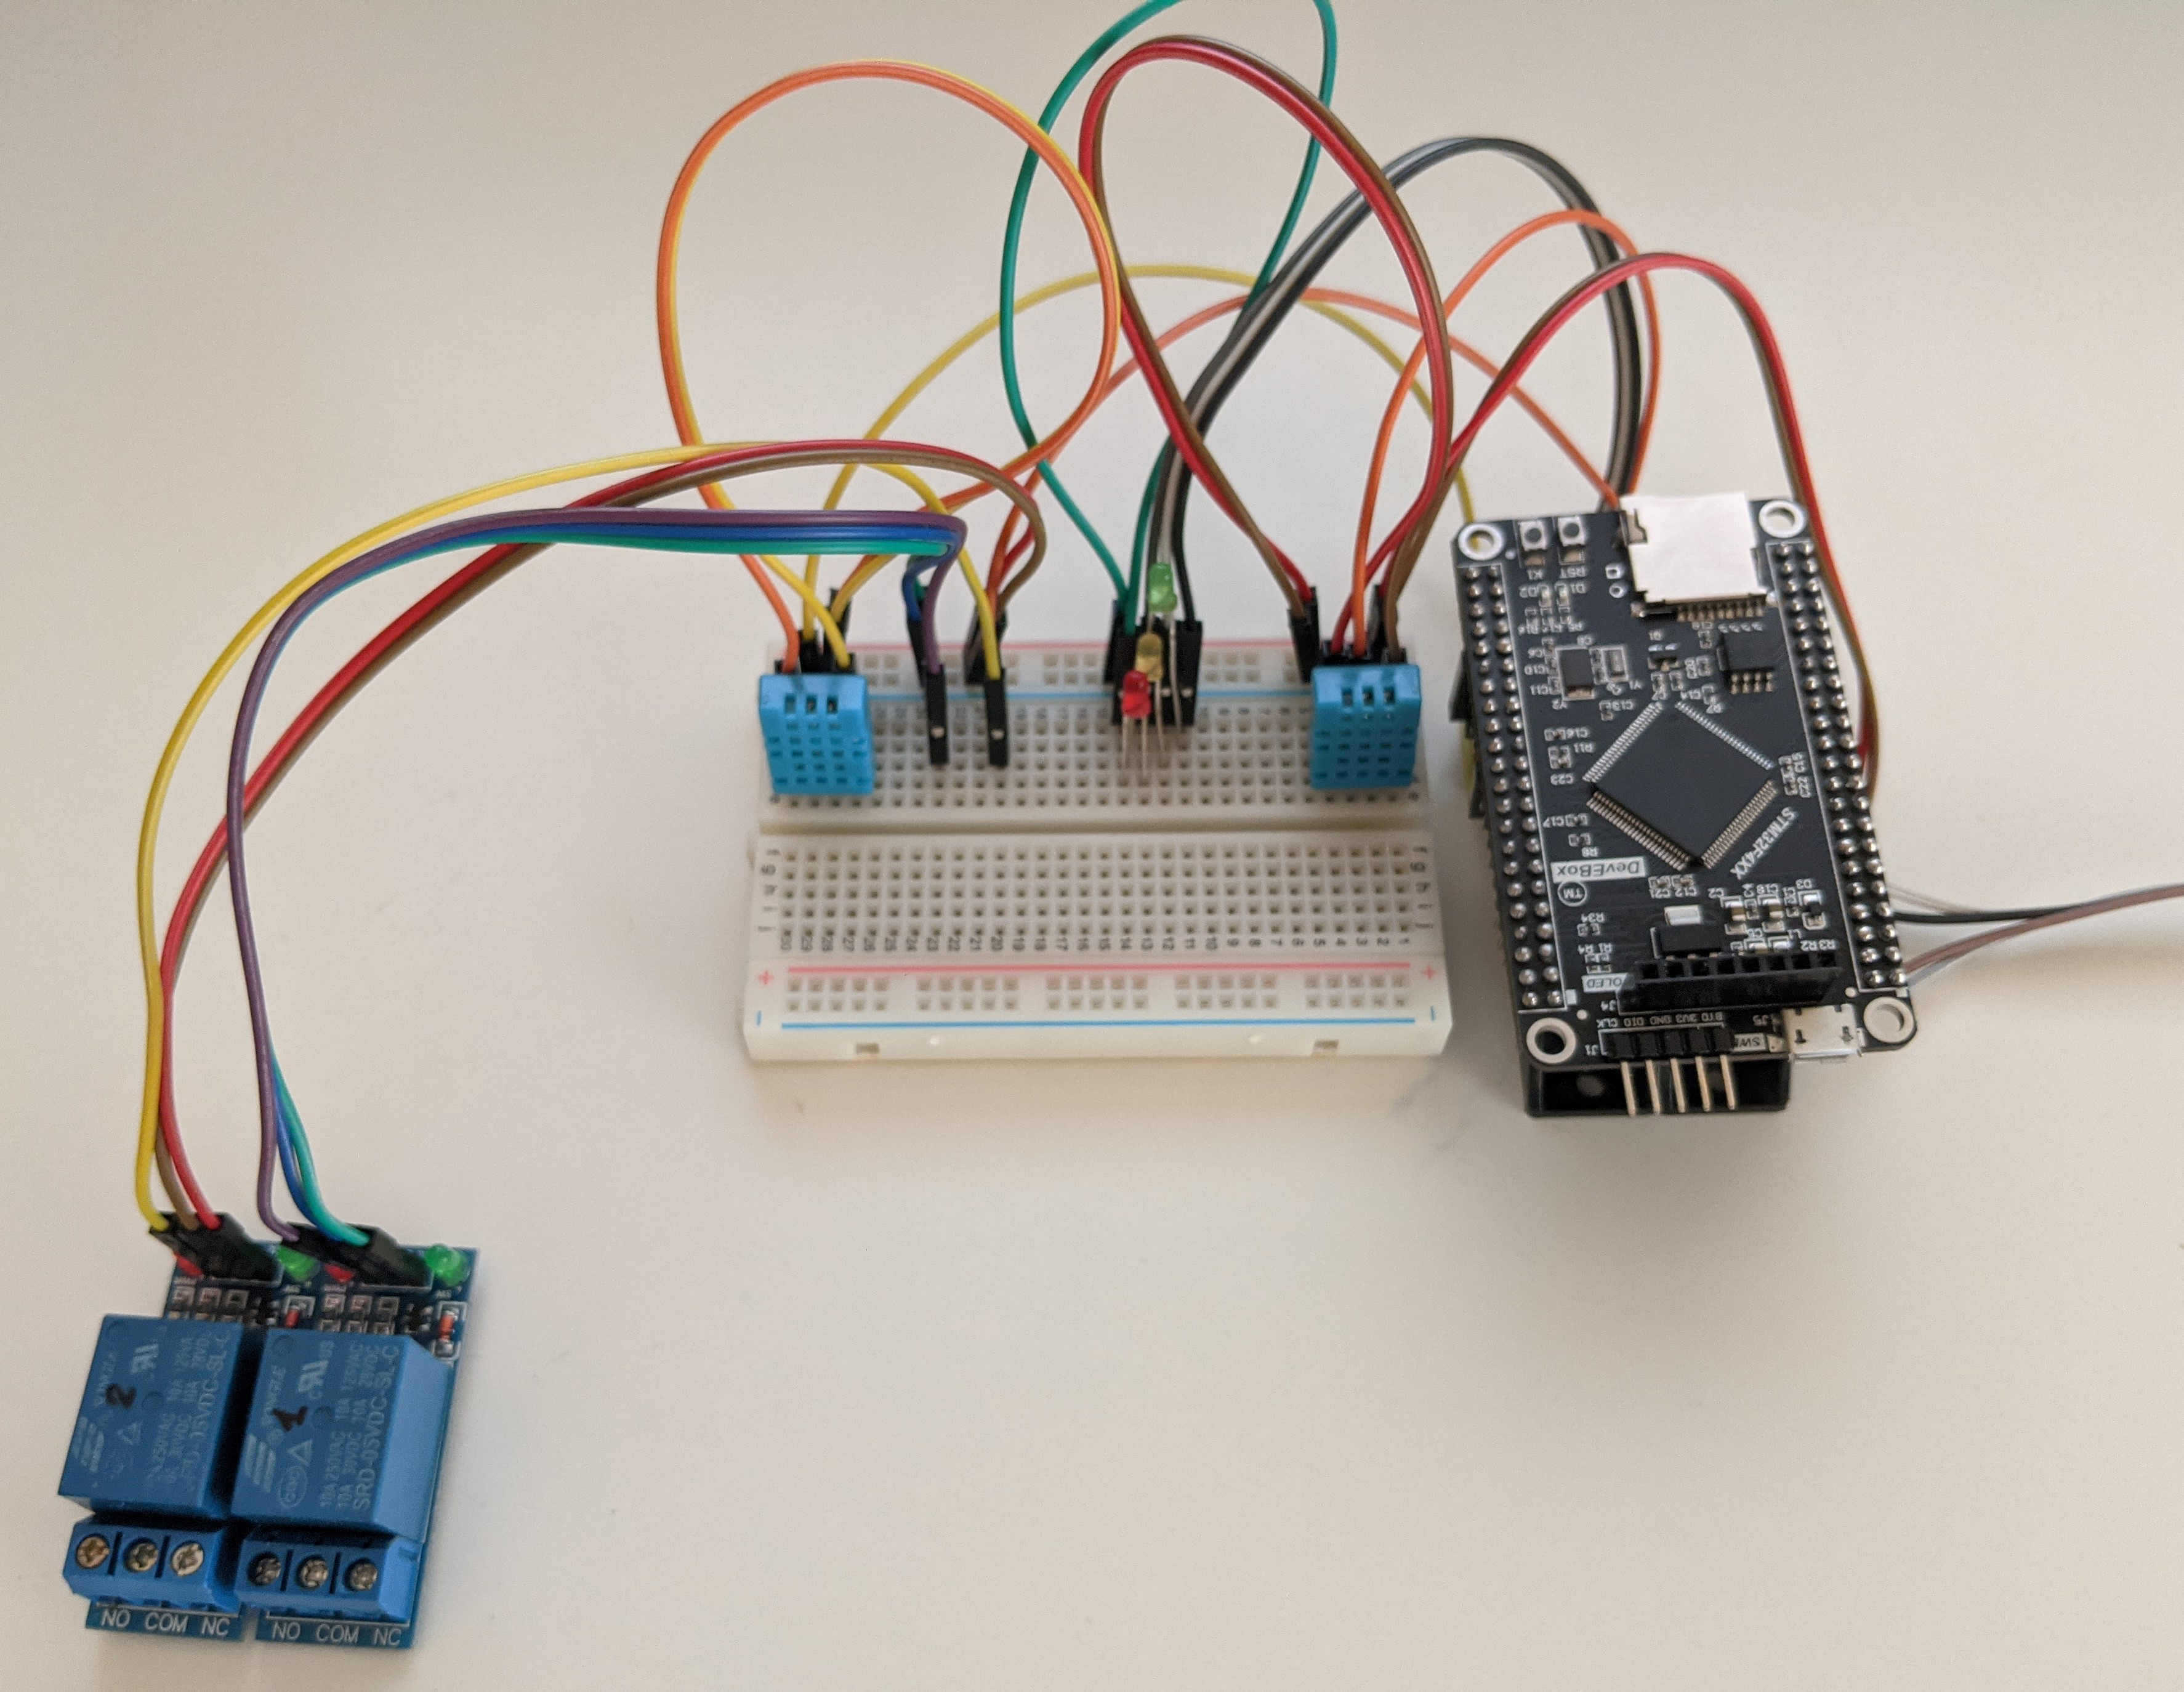
\includegraphics[width=0.7\columnwidth]{board_impl} 
	\caption{Board Implementation}
	\label{fig:board_impl}
\end{figure}

Looking ahead, thanks to the large fields of application, \emph{Well-being Station}
has a great  margin of improvement in terms of additional features. At the moment
it is fully wired and this approach perfectly fits large or unique environments,
for example in commercial and fitness domains. But with little changes, all the
actuators and sensors could be connected remotely and wirelessly. In such a way
we can also increase their number to support multi-zone and multi-room control.
Regarding the usability, instead, we could add an output display, or better a
touchscreen. This would let obtain more detailed information about the
environment, both indoor and outdoor, and allow more interaction, in order to
customize some parameters, such as time slots or devices to be connected.
Another interesting feature could be the Internet connectivity, that could rely
on the embedded ethernet support. It can be exploited in order to keep in sync
the internal RTC and automatically recognise daylight saving time, setting the
operating mode according to it. This connection can also be used to upload
measurements to a cloud database, letting the user consulting them when not at
home or maybe to enhance the algorithms used to compute the comfort zone
values. Last but not least, all of this can be used for a mobile application to
have full and remote control of the system.

\begin{thebibliography}{1}
		\bibitem{leudsen_freymark} Leudsen and Freymark,
			\emph{FLL-Innenraumbegrünungsrichtlinien}, 2011
		\bibitem{indoor_comfort} Boeing Consult, \emph{Room indoor comfortableness} Available:
			\url{https://www.boeingconsult.com/Environment/room-climate.htm}.		 
		\bibitem{pnpoly_2021}W.~Randolph Franklin, \emph{PNPOLY - Point
			Inclusion in Polygon Test, 2018} Available: ECSE,
			\url{https://wrf.ecse.rpi.edu/Research/Short_Notes/pnpoly.html}.
			[Accessed: 10 Feb. 2021].
		\bibitem{renode} Renode, \emph{A development framework which accelerates IoT and
			embedded system development} Available: \url{https://renode.io/}.
		\bibitem{devebox}DevEBox, \emph{Board definition files} Available:
			\url{https://github.com/mcauser/MCUDEV_DEVEBOX_F407VGT6}.	
	\end{thebibliography}
\end{document}

